\subsection{Data acquisition and computing}
\label {sec:daq}

The Data Acquisition (DAQ)
\nomenclature{DAQ}{Data acquisition system}
is designed to collect data from the detector
in events that have passed the L1 trigger.
Once events have passed the L1, data stored 
in pipeline memories in the front end electronics
are pushed into the DAQ system by Front End Drivers
(FEDs) \nomenclature{FED}{Front end driver}.
Therefore, the DAQ system must be able to sustain
an input rate of 100 kHz and an input data flow of
roughly 100 GB/s from roughly 650 FEDs.
The readout 

while providing enough
computing power


\begin{figure}
  \centering
  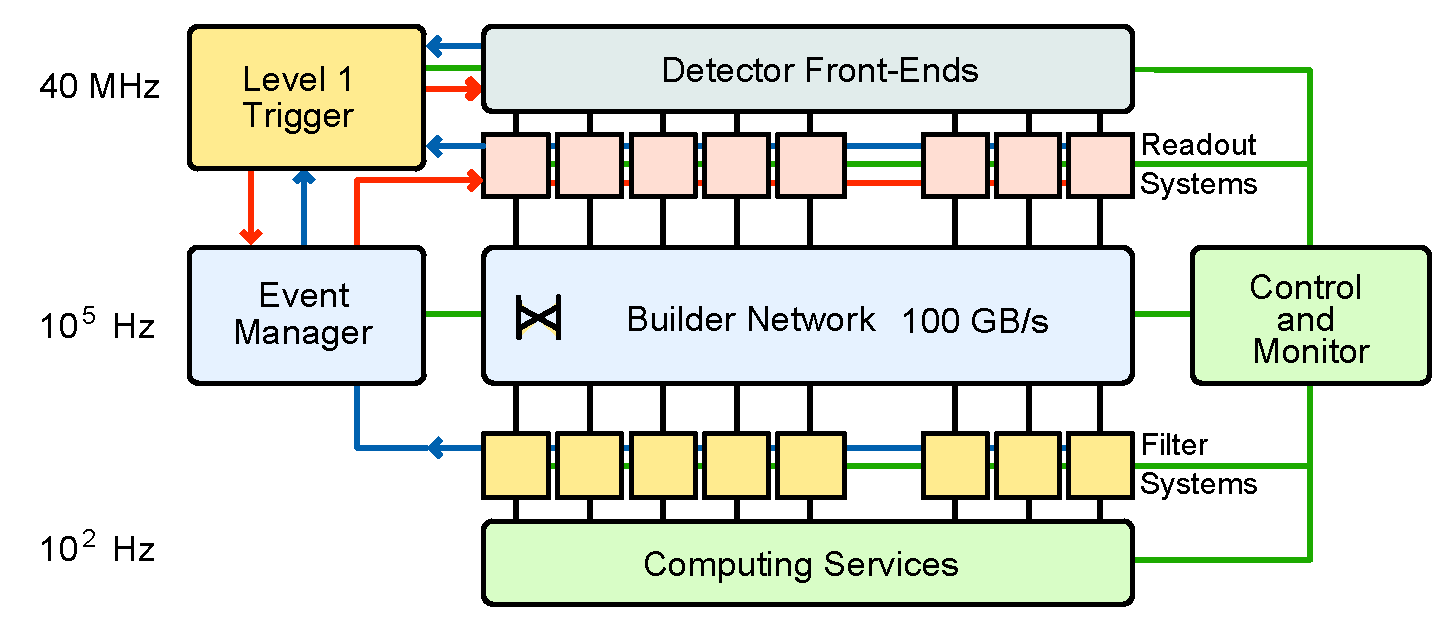
\includegraphics[width=0.6\textwidth]{tex/cms/fig/daq-schematic.pdf}
  \caption{Hello DAQ! \cite{cms-jinst}}
  \label{fig:daq}
\end{figure}
